\documentclass{article}

% if you need to pass options to natbib, use, e.g.:
%     \PassOptionsToPackage{numbers, compress}{natbib}
% before loading neurips_2020

% ready for submission
% \usepackage{neurips_2020}

% to compile a preprint version, e.g., for submission to arXiv, add add the
% [preprint] option:
%     \usepackage[preprint]{neurips_2020}

% to compile a camera-ready version, add the [final] option, e.g.:
     \usepackage[final]{neurips_2020}

% to avoid loading the natbib package, add option nonatbib:
%     \usepackage[nonatbib]{neurips_2020}

\usepackage[utf8]{inputenc} % allow utf-8 input
\usepackage[T1]{fontenc}    % use 8-bit T1 fonts
\usepackage{hyperref}       % hyperlinks
\usepackage{url}            % simple URL typesetting
\usepackage{booktabs}       % professional-quality tables
\usepackage{amsfonts}       % blackboard math symbols
\usepackage{nicefrac}       % compact symbols for 1/2, etc.
\usepackage{microtype}      % microtypography
\usepackage{graphicx}
\usepackage{float}

\title{AI Project 2: Multi-label Classification on YouTube-8M}

% The \author macro works with any number of authors. There are two commands
% used to separate the names and addresses of multiple authors: \And and \AND.
%
% Using \And between authors leaves it to LaTeX to determine where to break the
% lines. Using \AND forces a line break at that point. So, if LaTeX puts 3 of 4
% authors names on the first line, and the last on the second line, try using
% \AND instead of \And before the third author name.

\author{
 KAR CHUN TEONG\\
518030990014\\
  Department of Computer Science\\
  Shanghai Jiao Tong University\\
  \texttt{teongkarchun@sjtu.edu.cn} \\
 \And
  MATSUNAGA TAKEHIRO \\
518030990028\\
	Department of Computer Science\\
  Shanghai Jiao Tong University\\
  \texttt{matsunagatakehiro@sjtu.edu.cn} \\
\And
  EDUARDO WANG ZHENG \\
	518030990025\\
	Department of Computer Science\\
  Shanghai Jiao Tong University\\
  \texttt{eduardowangzheng@sjtu.edu.cn} \\
}


\begin{document}

\maketitle

\begin{abstract}
  The authors develop three models, which are Deep Fully Connected Neural Networks with Merge-and-Run Mappings(DMRNets), long short-term memory(LSTM), and bidirectional long short-term memory(biLSTM), to achieve multi-label classification on the YouTube-8M dataset.
\end{abstract}

\section{Introduction}
This project is the group project of CS410 Artificial Intelligence 2020 Fall in Shanghai Jiao Tong University named Multi-label Classification on YouTube-8M. The main purpose is to use a neural network model taking two video-level features(mean\_rgb and mean\_audio) as input, to output the prediction of labels of videos from the YouTube-8M dataset. The authors develop three different neural network models, which are DMRNets, LSTM and biLSTM in their attempts to achieve this goal.

\section{Methods}
\subsection{Deep Fully Connected Neural Networks with Merge-and-Run Mappings(DMRNets)}
\subsubsection{Model Overview}
One of the neural network architecture we consider is the deep fully connected neural networks with merge-and-run mappings, this is actually a variation of the deep convolutional neural networks with merge-and-run mappings, which coincidentally has the same short-form as DMRNets, to differentiate these two architectures, we would use DMRNets(FCN) as the short-form of Deep fully connected neural networks with Merge-and-Run Mappings and DMRNets(CNN) as the short-form of Deep convolutional neural networks with Merge-and-Run Mappings. DMRNets(CNN) itself is a variation of the residual neural network (ResNet). 

ResNet originated from Deep Convolutional Neural Networks(CNN), researchers have been pondering at the question of, does stacking more convolutional layers (which is increasing the depth) leads to better performance? They found out that stacking layers leads to a degradation problem, as they increase the depth, accuracy get saturated then degrades rapidly, and this is not caused by overfitting, the more layers they stack, the higher the training error. Some proposed a solution which is residual mapping, the basic building block of residual mapping is shown in Figure 1. Denote the desired underlying mapping as $H(x) = F(x) + x$, instead of directly fitting to $H(x)$, fit the layer to $F(x)$, and fit another layer to the identity mapping which is $x$, at the end merge the two layers to get the desired mapping $H(x)$. The authors of the article argued and proved that this modification significantly reduced the degradation problem while increasing the depth of the model, for more information please refer to the original article[1].

\begin{figure} [H]
  \centering
  \fbox{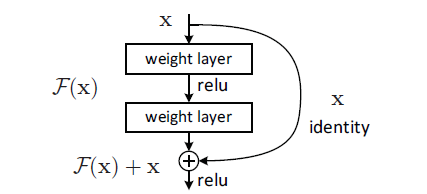
\includegraphics{Residual learning.png}}
  \caption{Residual Learning: a building block.}
\end{figure}

Next, we move on to the variation based on ResNet, the DMRNets(CNN). The idea behind this architecture is to assemble the residual branches in parallel through a merge-and run mapping. Merge means to average the inputs of these residual branches, and by Run it means to add the average to the output of each residual branch as the input of the subsequent residual branch.
To further illustrate the model, please refer to Figure 2. Figure 2(a) shows 2 residual branches assembled sequentially, Figure 2(b) shows 2 residual branches assembled in parallel and with identity mappings, and finally Figure 2(c) shows 2 residual branches assembled in parallel and with the proposed merge-and-run mappings. The authors of the article argued and proved that this modification further reduced the training difficulty of ResNet and retained the advantages of ResNet, for more information please refer to the original article[2].

\begin{figure} [H]
  \centering
  \fbox{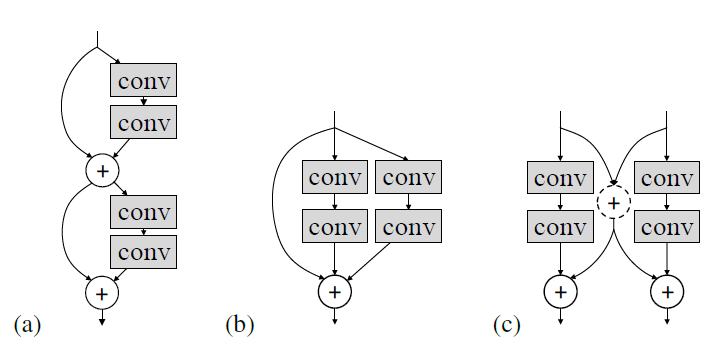
\includegraphics{DMRNets.png}}
  \caption{Comparison between different assembly blocks.}
\end{figure}

In this project, we adopt and do some variations on the DMRNets(CNN) by using the fully connected layers instead of convolutional layers as the basic layers to form the DMRNets(FCN). Part of the model structure is shown in Figure $3$. First we define a fc\_block which consists of dense layer, batch normalization layer, leaky ReLU layer, and dropout layer. Then we define the merge-and-run function, which separate input into 2 branches, branch a pass through the fc\_block while branch b pass through identity mapping, which is essentially mapping to itself, then we pass both branches into an average layer, then the output passes through another leaky ReLU layer. In Figure 3, we can see both input first go through a fc\_block, then into a merge-and-run mappings. The model is actually so deep that the rest of the structure is too large to be shown in the report, but it’s essentially the same process, repeatedly pass through fc\_block and merge-and-run mappings and finally merged into a single output, and the full picture is included in the submission folder.

 \begin{figure} [H]
  \centering
  \fbox{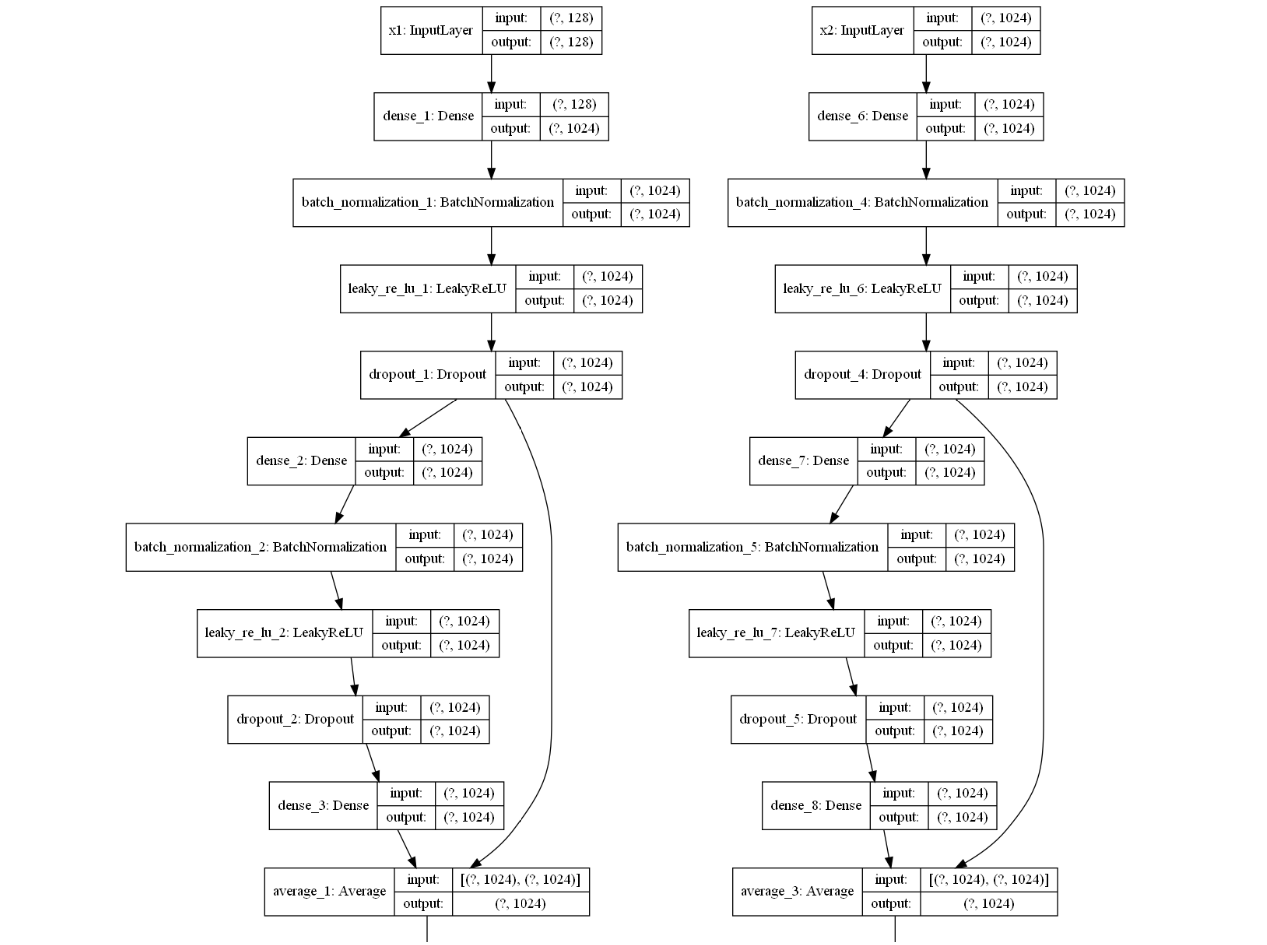
\includegraphics[width=16cm, height=15cm]{part of model structure(DMRNets).png}}
  \caption{Part of the structure of DMRNets(FCN).}
\end{figure}


\subsection{Long short-term memory (LSTM)}
\subsubsection{Model Overview}
Long short-term memory(LSTM) is a type of recurrent neural network (RNN) architecture,which is one of the most useful RNN.  Before LSTM, let's first talk about RNN, the structure of a typical RNN is shown in Figure 4. As our brain can understand articles based on knowledge that we learned before, RNN works in a similar way, RNN can derive some parameters from its forward node, this was what traditional neural networks could not achieve. However, traditional RNN could not store what it learned from forward node for a dragged time period, since every cell of RNN will process both input and derived information in activation function, but LSTM solved this problem. Beside forward outputs, another data is derived from forward nodes in LSTM network. The increasing data will only interact with a few data that processed in cell, which means it will keep the knowledge that it learned for a long time.
\begin{figure}[H]
  \centering
  \fbox{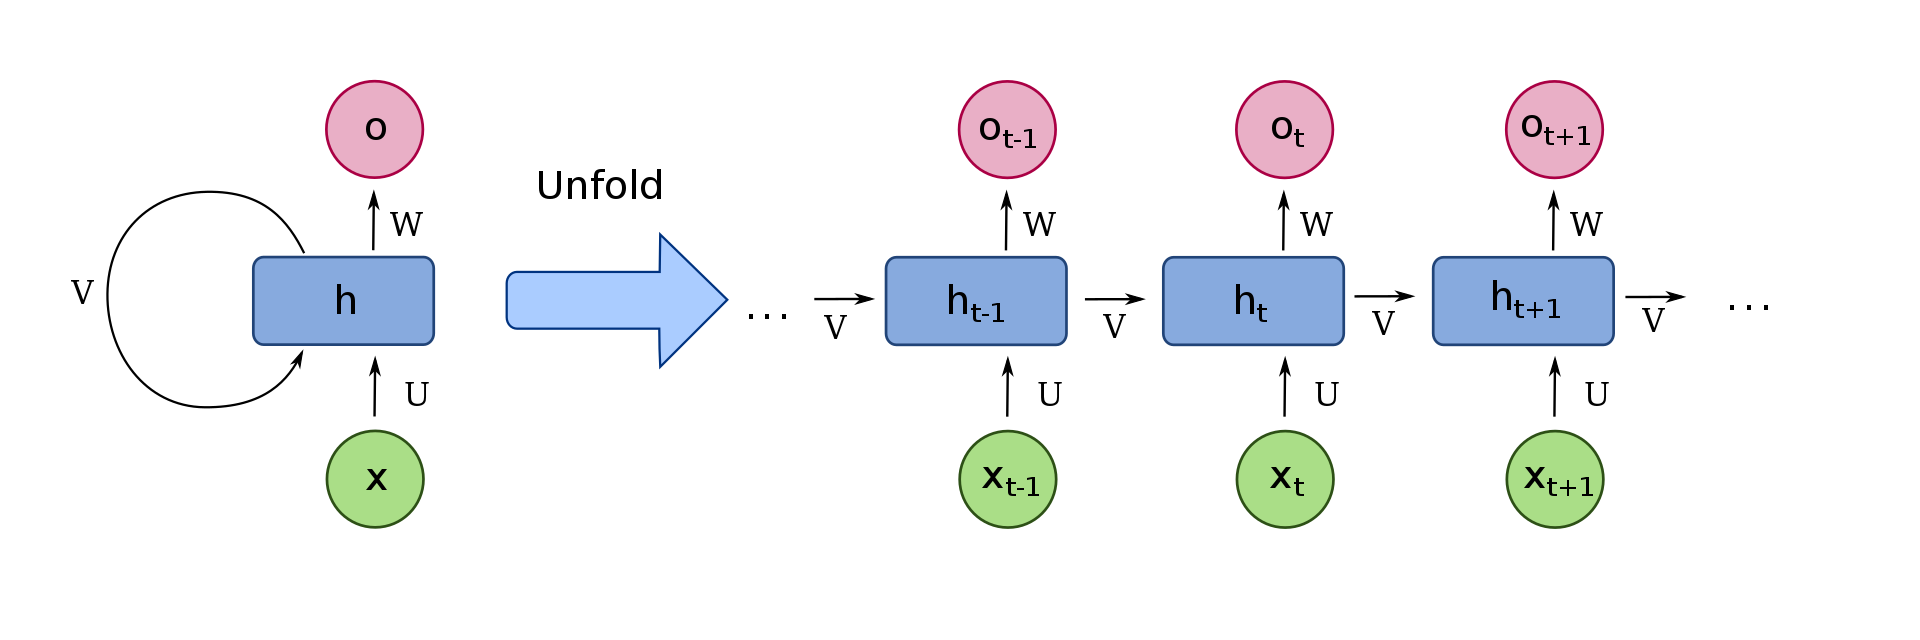
\includegraphics[width=14cm, height=5cm]{RNN.png}}
  \caption{Structure of RNN}
\end{figure}

A common LSTM unit is composed of a cell and 3 gates. The cell stores values over time intervals as cell states, and the 3 gates’ main job is to regulate the flow of information into and out of the cell. Specifically, forget gate decides which information to forget, input gate decides to update which value of cell states and update cell states, and at last, the output gate output filtered cell states. The structure of a LSTM cell is shown in Figure 5. To put it in an abstract high-level view, what LSTM do is using past context as reference to predict the output, for more information please refer to the original article[3].

Each step in the forget gate of a LSTM cell is shown below:
\begin{itemize}
\item step1: $f_t = \sigma(W_f[h_{t-1}, x_t] + b_f)$
\item step2: $i_t = \sigma(W_i[h_{t-1}, x_t] + b_i)$,  $\widetilde{C} = tanh(W_C[h_{t-1}, xt] + b_C)$
\item step3: $o_t=\sigma(W_o[h_{t-1}, x_t] + b_o)$
\item step4: $C_t = f_t*C_{t-1} + i_t*\widetilde{C}$
\item step5: $h_t=o_t*tanh(C_t)$
\end{itemize}
\begin{figure}[h]
  \centering
  \fbox{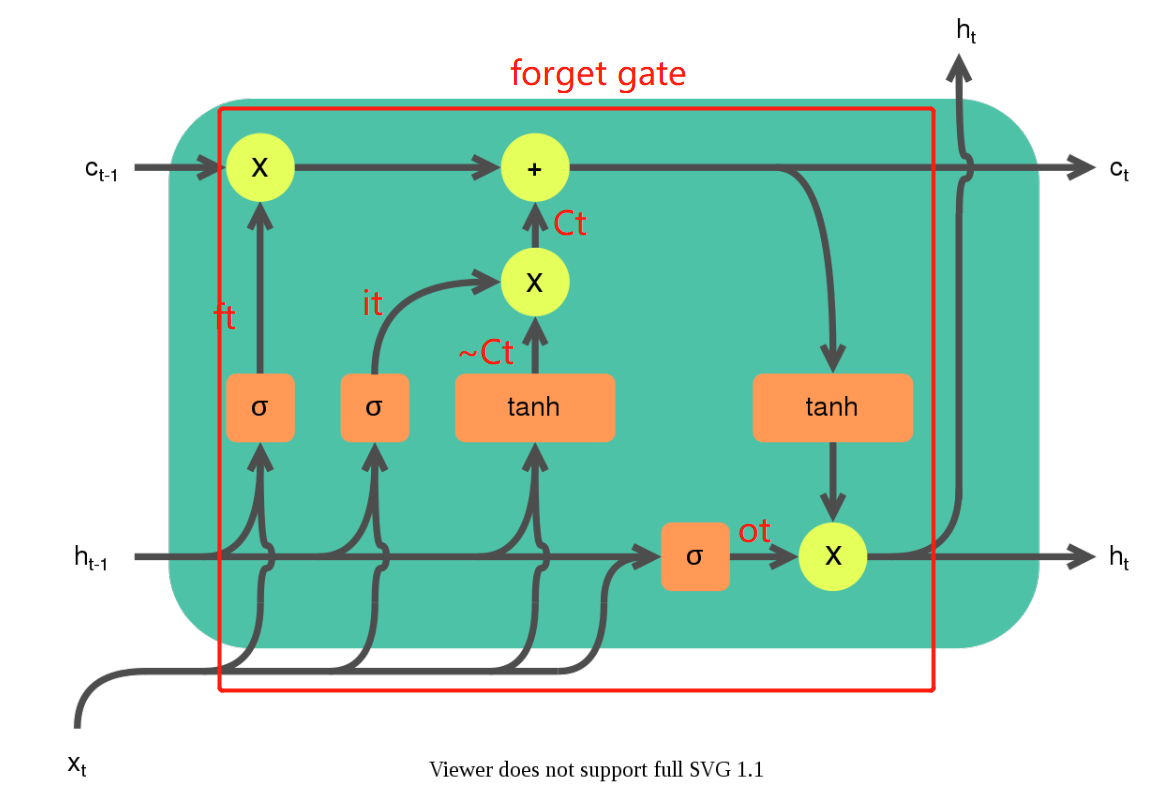
\includegraphics[width=12cm, height=8cm]{lstm1.png}}
  \caption{Structure of LSTM}
\end{figure}


\subsection{Bidirectional Long short-term memory (biLSTM)}
\subsubsection{Model Overview}
biLSTM is a variant of LSTM, biLSTM train two instead of one LSTMs on one input sequence, the first on the input sequence, and the second on a reversed copy of the input sequence. In other words, it connects two hidden layers of opposite directions to the same output, this generally provide additional context to the network, thus results in better training results. The structure of biLSTM is shown in Figure 6, for more information please refer to the original article[4].
\begin{figure}[h]
  \centering
  \fbox{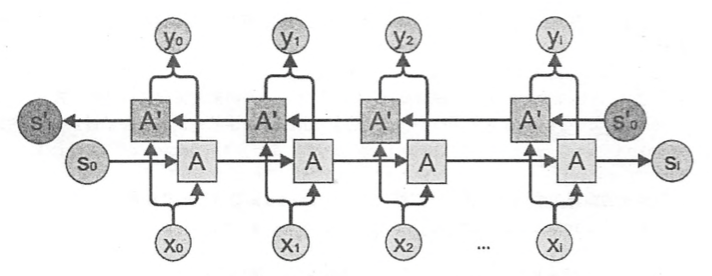
\includegraphics[width=16cm, height=7cm]{biLSTM.png}}
  \caption{Structure of biLSTM}
\end{figure}

In our project, we train two features separately in two biLSTM cells, then merge them together, the model structure is shown in Figure 7. The model first extends the mean\_RGB features to 1024. Processing the data by using batch normalization and reshape in order pass the data into the bidirectional LSTM cell. Then, the model use dropout to mix some noise into the data to prevent overfitting. We do the same for the mean\_audio features. And finally we concatenate the two features into one output, and pass them through some final layers. The model structure is shown in Figure 7.
\begin{figure}[h]
  \centering
  \fbox{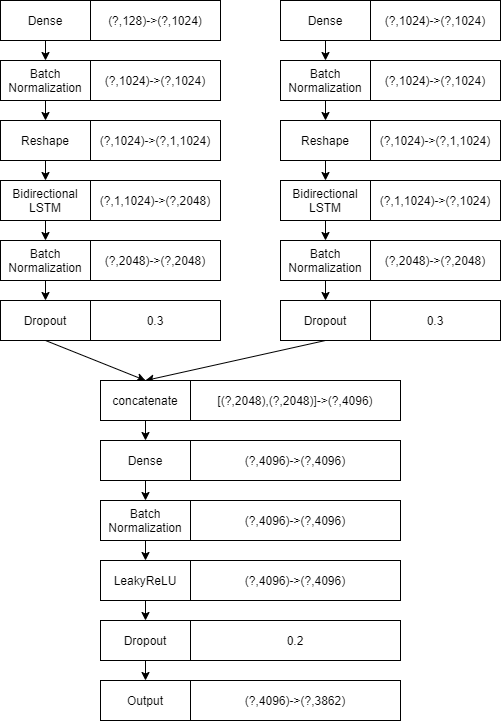
\includegraphics[width=10cm, height=14cm]{bilstm_structure.png}}
  \caption{Model structure of biLSTM}
\end{figure}

\section{Experiments and Analysis}
\subsection{Training}
We wanted to use cloud platforms to train our model, but most of them needs payment, and we don't have the fund for that, Google Cloud Platform offers 1 month free trial, but to get the free trial we need to register with credit card, which unfortunately we don't possess, at the end of the day we need to train the model using our local machines. Limited by the performance of our local machines, we could only use a small subset of the datasets for training, in this case, we use the first 200 training shards (train0000.tfrecord~train0199.tfrecord) and the first 100 validation shards (validate0000.tfrecord~validate0099.tfrecord) as our training datasets. Figure 8 and 9 shows the graph of training curve of the LSTM and biLSTM models. As shown in the figures, both models converged at around $0.75$, with biLSTM having a slightly better performance.

\begin{figure}
  \centering
  \fbox{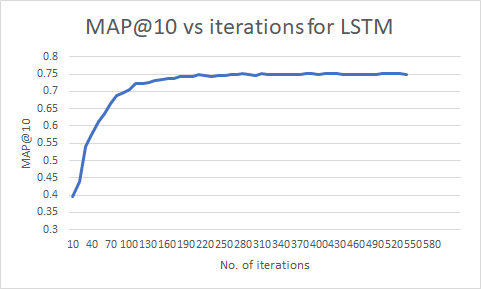
\includegraphics[width=10cm, height=6cm]{lstm graph.png}}
  \caption{LSTM training graph}
\end{figure}

\begin{figure}
  \centering
  \fbox{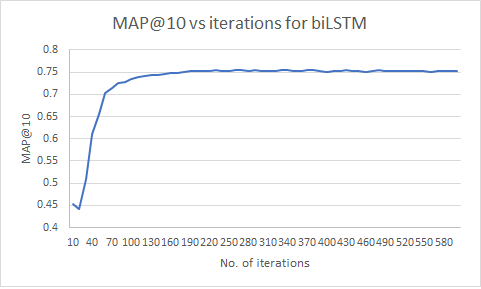
\includegraphics[width=10cm, height=6cm]{bilstm graph.png}}
  \caption{biLSTM training graph}
\end{figure}

For unknown reasons, the training of the DMRNets model did not converge, we tried modifying various parameters and adjusting the depth of the model, but in the end it couldn't work.

\subsection{Comparison and Analysis of Performance}
\begin{table} [H]
  \caption{Performance of different models}
  \label{table 1}
  \centering
  \begin{tabular}{llll}
    \toprule
    Model     & 200 train MAP@10     & 100 validation MAP@10 & All datasets MAP@10 \\
    \midrule 
LSTM & 0.935  & 0.946 & 0.759     \\
biLSTM     & 0.949 & 0.961 & 0.764      \\
    \bottomrule
  \end{tabular}
\end{table}
The performances of 2 models are listed in Table \ref{table 1}, as we could see, the MAP@10 for the first 200 training shards and 100 validation shards are always significantly higher than the MAP@10 for the whole datasets, the reason is obvious as we use the first 200 training shards and 100 validation shards as training datasets which leads to possible overfitting. However, we consider that the LSTM and biLSTM's performance of around 0.75 to 0.76 for the whole datasets as satisfactory, since we only use an extremely small subset to train them. We hypothesize that if we use larger datasets for training, the model would lead to more satisfactory results, too bad that we don't have the computing power to prove this hypothesis.

\section{Conclusion}
Based on the experiments, we conclude that the biLSTM model has a superior performance over the other models we used. Therefore we use the biLSTM model in our final submission. However, we also submit the other models along the submission files as supplement materials for grading purpose.

The corresponding files to each models in the submission folder are shown below:
\begin{enumerate}
\item LSTM model: LSTM\_model.py and LSTM\_train.py
\item biLSTM model: biLSTM\_model.py, train.py, and test.py
\end{enumerate}

\section{Contributions}
\begin{itemize}
\item KAR CHUN TEONG: 
\begin{itemize}
\item Production management(organization and distribution of workload, arrangement of meeting schedule, etc.)
\item Analysis and implementation of DMRNets model
\item Design, creation, and compilation of final report and PPT
\end{itemize}
\item MATSUNAGA TAKEHIRO
\begin{itemize}
\item Analysis and implementation of LSTM and biLSTM model
\item Training and testing of LSTM and biLSTM model
\end{itemize}
\item EDUARDO WANG ZHENG
\begin{itemize}
\item Research for other models
\end{itemize}
\end{itemize}

\section{References}
\medskip

\small

[1] Kaiming He, Xiangyu Zhang, Shaoqing Ren, Jian Sun. Deep Residual Learning for Image Recognition.

[2] Liming Zhao, Mingjie Li, Depu Meng, Xi Li, Zhaoxiang Zhang. Deep Convolutional Neural Networks with Merge-and-Run Mappings.

[3] Sepp Hochreiter. Long Short-Term Memory. 

[4] Alex Graves, Jürgen Schmidhuber. Framewise phoneme classification with bidirectional LSTM and other neural network architectures. 


\section{Afterwords}
Other than the three models we analysed and used in the report, there are numerous models we attempted to use for this project. However, they either fail miserably in terms of performance, or they couldn't be implemented effectively for the project's purpose. And due to the limitation on length of the report, we couldn't include all the models we tried in this report.

The coordination and organization of group works for members who lived in different countries are difficult than imagined, the network helps for sure but we still believe that the hurdle for our group is higher than the rest. To make the matters worse, a group member we didn't list in the title and contribution parts, Yernur Kassymov, actually joined in our group halfway in the process, declaring that he didn't join a group months ago, we thought that we are the only group with three members so it was fine, but it was wrong. Inspite of our weekly reminder of the pending work at his end, he did not finish his job and declared to take a gap year from school one week before the submission date, which essentially rendered this project useless to him since the grade would not matter to him anymore. However, the rest of the group members had to pick up the job left by him within one week, this heavily tolls on the progress and quality of our work. Pointing fingers is not our intention but we could not let it slides without any mention on this infuriating act which is a heavy violation on work ethics.
\end{document}



